\chapter{Visión general del acceso a datos textuales}\label{Chapter3}
% chktex-file 8
% chktex-file 12
% chktex-file 13
% chktex-file 44

El acceso a datos textuales es la base para el análisis de texto. La tecnología de acceso a texto desempeña dos roles importantes en las aplicaciones de gestión y análisis de texto. Primero, permite la recuperación de los datos textuales más relevantes para un problema de análisis particular, evitando así el procesamiento innecesario de una gran cantidad de datos no relevantes. Segundo, permite la interpretación de cualquier resultado de análisis o conocimiento descubierto en el contexto adecuado y proporciona la procedencia de los datos (origen). \\

El objetivo general del acceso a datos textuales es conectar a los usuarios con la información correcta en el momento adecuado. Esta conexión se puede realizar de dos maneras: \textit{pull}, donde los usuarios toman la iniciativa de extraer información relevante del sistema, y \textit{push}, donde el sistema toma la iniciativa de ofrecer información relevante a los usuarios.

\section{Modos de acceso: \textit{pull} y \textit{push}}

Dado que los datos textuales son creados para ser consumidos por humanos, estos últimos juegan un papel importante en las aplicaciones de análisis y gestión de datos textuales. Específicamente, los humanos pueden ayudar a seleccionar los datos más relevantes para un problema particular, lo cual es beneficioso al permitir evitar procesar la gran cantidad de datos textuales crudos (lo cual sería ineficiente) y centrarse en analizar la parte más relevante. Seleccionar datos textuales relevantes de una gran colección es la tarea básica del acceso a texto. Esta selección generalmente se basa en una especificación de la necesidad de información de un analista (un usuario), y se puede hacer en dos modos: pull y push. La figura \ref{fig:5.1} describe cómo estos modos se ajustan junto con la consulta y la navegación. \\

\begin{figure}[h]
\centering
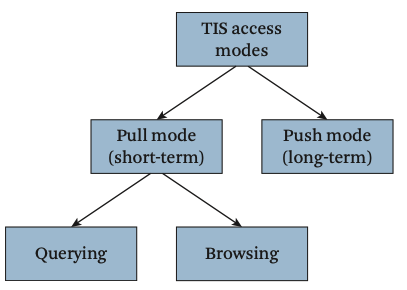
\includegraphics[width=0.4\textwidth]{fotos/12.png}
\caption{La dicotomía de los modos de acceso a la información textual.}
\label{fig:5.1}
\end{figure}

\subsubsection{\textit{Pull}}

En el modo \textit{pull}, el usuario inicia el proceso de acceso para encontrar los datos textuales relevantes, típicamente utilizando un motor de búsqueda. Este modo de acceso a texto es esencial cuando un usuario tiene una necesidad de información \textit{ad hoc}, es decir, una necesidad de información temporal que podría desaparecer una vez que se satisfaga la necesidad. Por ejemplo, un usuario puede tener la necesidad de comprar un producto y, por lo tanto, estar interesado en recuperar todas las opiniones relevantes sobre productos candidatos; después de que el usuario haya comprado el producto, generalmente ya no necesitará dicha información. Otro ejemplo es que durante el proceso de análisis de datos de redes sociales para entender opiniones sobre un evento emergente, el analista también puede decidir explorar información sobre una entidad particular relacionada con el evento (por ejemplo, una persona), lo que también puede desencadenar una actividad de búsqueda. \\

Si bien la consulta es la forma más común de acceder a datos textuales en el modo \textit{pull}, la navegación es otra forma complementaria de acceder a datos textuales en el modo \textit{pull}, y puede ser muy útil cuando un usuario no sabe cómo formular una consulta efectiva, o encuentra inconveniente ingresar una consulta de palabras clave (por ejemplo, a través de un teléfono inteligente), o simplemente quiere explorar un tema sin un objetivo fijo. De hecho, al buscar en la \textit{web}, los usuarios tienden a mezclar la consulta y la navegación (por ejemplo, al atravesar hipervínculos). En general, se puede considerar la consulta y la navegación como dos formas complementarias de encontrar información relevante en el espacio de información y, cuando la consulta no funciona bien, la navegación puede ser muy útil. 

\subsubsection{\textit{Push}}

En el modo \textit{push}, el sistema inicia el proceso para recomendar un conjunto de elementos de información relevantes al usuario. Este modo de acceso a la información es generalmente más útil para satisfacer una necesidad de información a largo plazo de un usuario o analista, como pueden ser los intereses de investigación de un investigador, que pueden considerarse relativamente estables a lo largo del tiempo. En comparación, el flujo de información (es decir, los artículos de investigación publicados) es dinámico. Aunque un usuario puede buscar regularmente información relevante con consultas, es más deseable que un sistema de recomendación (también llamado sistema de filtrado) monitoree el flujo de información dinámico y "empuje" cualquier artículo relevante al usuario basado en la coincidencia de los artículos con los intereses del usuario (por ejemplo, en forma de un correo electrónico). \\

Otro escenario del modo \textit{push} es la recomendación iniciada por el productor (difusión selectiva de información, SDI). En este escenario, el productor de información tiene interés en difundir la información entre los usuarios relevantes, y empujaría un elemento de información a dichos usuarios. La publicidad de información de productos en las páginas de resultados de búsqueda es un ejemplo de esto. La recomendación puede entregarse a través de notificaciones por correo electrónico o recomendarse a través de una página de resultados de un motor de búsqueda. 

\subsubsection{Necesidad de información}

En términos generales, hay dos tipos de necesidades de información: a corto y a largo plazo. Las necesidades a corto plazo están a menudo asociadas con el modo \textit{pull}, y las necesidades a largo plazo están más asociadas con el modo \textit{push}. Una necesidad de información a corto plazo es temporal y generalmente se satisface a través de la búsqueda o navegación en el espacio de información, mientras que una necesidad de información a largo plazo puede satisfacerse mejor a través del filtrado o la recomendación, donde el sistema tomaría la iniciativa de empujar la información relevante a un usuario. \\

La recuperación \textit{ad hoc} es extremadamente importante porque las necesidades de información \textit{ad hoc} aparecen con mucha más frecuencia que las necesidades de información a largo plazo. Las técnicas efectivas para la recuperación \textit{ad hoc} generalmente pueden reutilizarse para el filtrado y la recomendación también. Además, en el caso de necesidades de información a largo plazo, es posible recopilar comentarios de los usuarios (\textit{feedback}), que pueden ser explotados. En este sentido, la recuperación \textit{ad hoc} es mucho más difícil, ya que no existe mucha información de retroalimentación de un usuario (es decir, pocos datos de entrenamiento para una consulta particular). Debido a la disponibilidad de datos de entrenamiento, el problema del filtrado o la recomendación generalmente puede resolverse utilizando técnicas de aprendizaje automático supervisado.

\section{Acceso interactivo multimodal}

Idealmente, el sistema debería proporcionar soporte para que los usuarios tengan acceso interactivo multimodal a datos textuales relevantes, de modo que los modos \textit{push} y \textit{pull} estén integrados en el mismo entorno de acceso a la información, y la consulta y la navegación también estén integradas sin problemas. Esto proporciona la máxima flexibilidad a los usuarios y les permitir consultar y navegar a voluntad. \\

\begin{figure}[h]
\centering
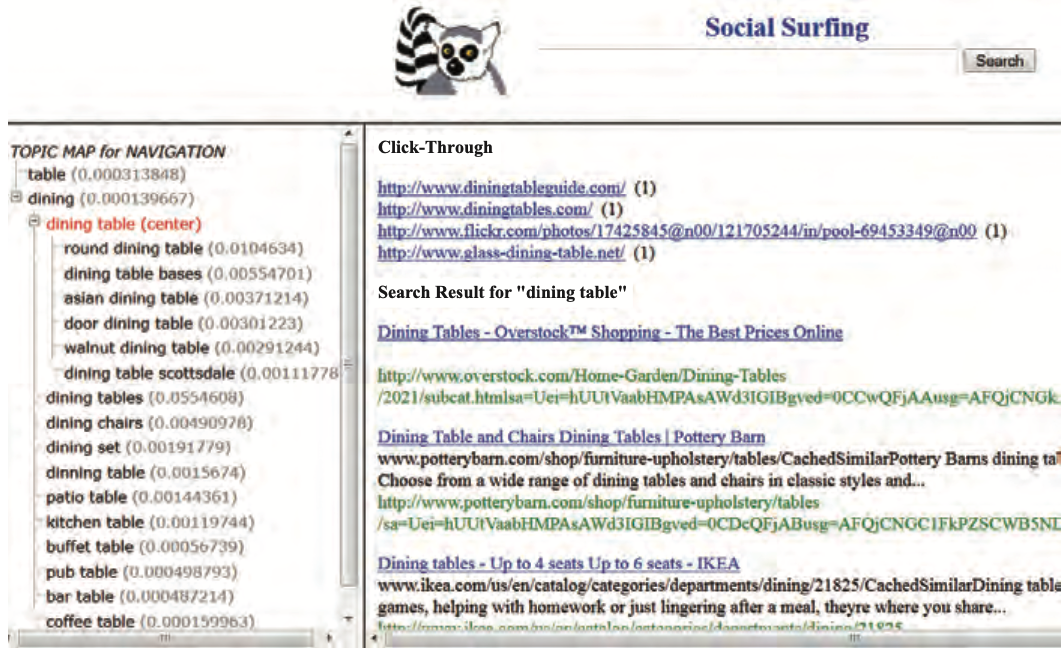
\includegraphics[width=0.6\textwidth]{fotos/13.png}
\caption{Ejemplo de interfaz de navegación con un mapa de temas donde la navegación y la consulta están integradas de manera natural.}
\label{fig:5.2}
\end{figure}

En la figura \ref{fig:5.2} se tiene un sistema prototipo donde se ha añadido un mapa de temas construido automáticamente basado en un conjunto de consultas recopiladas en un motor de búsqueda comercial a una interfaz de motor de búsqueda regular para permitir que un usuario navegue por el espacio de información de manera flexible. Con esta interfaz, un usuario puede hacer cualquiera de las siguientes acciones en cualquier momento: 
\begin{itemize}
\item Consulta (salto de largo alcance). Cuando un usuario envía una nueva consulta a través del cuadro de búsqueda, los resultados de un motor de búsqueda se muestran en el panel derecho. Al mismo tiempo, la parte relevante de un mapa de temas también se muestra en el panel izquierdo para facilitar la navegación si el usuario lo desea.
\item Navegación en el mapa (caminata de corto alcance). El panel izquierdo de la interfaz permite que un usuario navegue por el mapa. Cuando un usuario hace clic en un nodo del mapa, este panel se actualizará y se mostrará una vista local con el nodo clicado como el foco actual. En la vista local, mostramos los padres, los hijos y los vecinos horizontales del nodo actual en foco (etiquetado como "centro" en la interfaz). Un usuario puede así hacer \textit{zoom} en un nodo hijo, hacer \textit{zoom} hacia afuera a un nodo padre, o navegar a un nodo vecino horizontal. El número adjunto a un nodo es una puntuación para el nodo que usamos para clasificar los mismos. Dicho mapa permite al usuario ``caminar'' en el espacio de información para navegar por documentos relevantes sin necesidad de reformular consultas.
\item Visualización de una región temática. El usuario puede hacer doble clic en un nodo temático en el mapa para ver los documentos cubiertos en la región temática. El panel de resultados de búsqueda se actualizaría con nuevos resultados correspondientes a los documentos en la región temática seleccionada. 
\item Visualización de un documento. Dentro del panel de resultados, un usuario puede seleccionar cualquier documento para verlo como en una interfaz de búsqueda estándar.
\end{itemize}

En la figura \ref{fig:5.3}, se muestra un ejemplo de traza de navegación en la que el usuario comenzó con una consulta ``\textit{dining table}'', hizo \textit{zoom} en ``\textit{asian dining table}'', hizo \textit{zoom} hacia afuera de nuevo a ``\textit{dining table}'', navegó horizontalmente primero a ``\textit{dining chair}'' y luego a ``\textit{dining furniture}'', y finalmente hizo \textit{zoom} hacia afuera al tema general ``\textit{furniture}'' donde el usuario tendría muchas opciones para explorar diferentes tipos de muebles. Si este usuario siente que se necesita un ``salto largo'', puede usar una nueva consulta para lograrlo. Dado que el mapa puede ocultarse y solo mostrarse cuando el usuario lo necesita, dicha interfaz es una extensión muy natural de la interfaz de búsqueda actual desde la perspectiva del usuario. Así, se puede ver cómo un sistema de acceso a texto puede combinar múltiples modos de acceso a la información para adaptarse a las necesidades actuales de un usuario.

\begin{figure}[h]
\centering
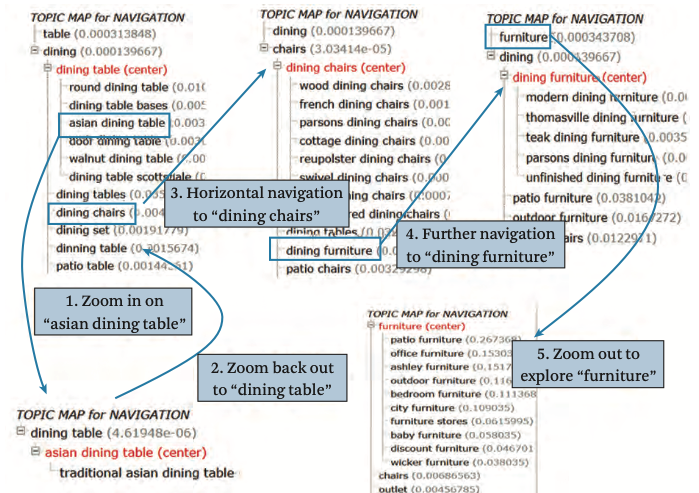
\includegraphics[width=0.6\textwidth]{fotos/14.png}
\caption{Ejemplo de traza de navegación en un mapa de temas, sin necesidad de hacer consultas.}
\label{fig:5.3}
\end{figure}

\section{Recuperación de texto}

La herramienta más importante para apoyar el acceso a datos textuales es un motor de búsqueda (SE). Estos proporcionan soporte directo para la consulta y pueden extenderse fácilmente para proporcionar recomendaciones o navegación. Además, las técnicas utilizadas para implementar un motor de búsqueda efectivo a menudo también son útiles para la implementación de un sistema de recomendación, así como para muchas funciones de análisis de texto. \\

Desde la perspectiva del usuario, el problema de la TR es usar una consulta para encontrar documentos relevantes en una colección de documentos de texto. Esta es una tarea necesaria de forma frecuente, ya que los usuarios a menudo tienen necesidades de información \textit{ad hoc} temporales para varias tareas, y necesitan encontrar la información relevante de inmediato. El sistema para apoyar la TR es un sistema de recuperación de texto, o un motor de búsqueda. \\

Aunque la TR a veces se usa indistintamente con el término más general ``recuperación de información'' (IR), este último también incluye la recuperación de otros tipos de información, como imágenes o videos. Sin embargo, las técnicas de recuperación para otros datos no textuales son menos maduras y, como resultado, la recuperación de esta tiende a depender del uso de técnicas de recuperación de texto para hacer coincidir una consulta de palabras clave con datos textuales acompañados de un elemento de datos no textuales. Por ejemplo, los motores de búsqueda de imágenes actuales en la \textit{web} son esencialmente un sistema de TR donde cada imagen está representada por un documento de texto que consiste en cualquier dato textual asociado con la imagen (por ejemplo, título, leyenda, etc). \\

La tarea de la TR puede ser más o menos complicada dependiendo de consultas específicas y colecciones específicas. Por ejemplo, durante una búsqueda \textit{web}, encontrar páginas de inicio generalmente es fácil, pero encontrar opiniones de personas sobre algún tema (por ejemplo, la política exterior de EE. UU.) sería más difícil. Hay varias razones por las cuales la TR es complicada:
\begin{itemize}
\item Una consulta suele ser bastante corta e incompleta (no es un lenguaje formal como SQL).
\item La necesidad de información puede ser difícil de describir con precisión, especialmente cuando el usuario no está familiarizado con el tema.
\item La comprensión precisa del contenido del documento es difícil. En general, dado que lo que cuenta como la respuesta correcta es subjetivo, incluso cuando los expertos humanos juzgan la relevancia de los documentos, pueden no estar de acuerdo entre sí.
\end{itemize}

Debido a la falta de estructuras semánticas claras y la dificultad en la comprensión del lenguaje natural, a menudo es un reto recuperar con precisión información relevante para la consulta de un usuario. De hecho, aunque los motores de búsqueda \textit{web} actuales pueden parecer suficiente, aún puede ser complicado para un usuario localizar y recolectar rápidamente toda la información relevante para una tarea. En general, los motores de búsqueda actuales funcionan muy bien para consultas de navegación y consultas informativas simples y populares, pero en el caso de que un usuario tenga una necesidad de información compleja, como analizar opiniones sobre productos para comprar o investigar información médica sobre algunos síntomas, a menudo funcionan mal. Además, los motores de búsqueda actuales generalmente proporcionan poco o ningún soporte para ayudar a los usuarios a digerir y explotar la información recuperada. Como resultado, incluso si un motor de búsqueda puede recuperar la información más relevante, un usuario aún tendría que revisar una larga lista de documentos y leerlos en detalle para digerir completamente el conocimiento enterrado en los datos textuales para realizar su tarea.

\section{Recuperación de texto vs recuperación de bases de datos}

Es útil hacer una comparación del problema de la recuperación de texto (TR) y el problema de la recuperación de bases de datos. Ambas tareas de recuperación son para ayudar a los usuarios a encontrar información relevante, pero debido a la diferencia en los datos gestionados por estas dos tareas, hay muchas diferencias importantes. \\

Primero, los datos gestionados por un motor de búsqueda y un sistema de bases de datos son diferentes. En las bases de datos, los datos están estructurados, cada campo tiene un significado claramente definido según un esquema. Por lo tanto, los datos pueden verse como una tabla con columnas bien especificadas. Por ejemplo, en un sistema de base de datos de un banco, un campo puede ser nombres de clientes, otro puede ser la dirección, y otro más puede ser el saldo de cada tipo de cuenta. En contraste, los datos gestionados por un motor de búsqueda son texto no estructurado que puede ser difícil de entender para los ordenadores. Así, incluso si una oración dice que una persona vive en una dirección particular, sigue siendo difícil para el ordenador responder una consulta sobre la dirección de una persona en respuesta a una consulta de palabras clave, ya que no hay una estructura definida simple para el texto libre. Aquí es el sistema el que debe ver qué es relevante en cada búsqueda. \\

En segundo lugar, una consecuencia de la diferencia en los datos es que las consultas que pueden ser soportadas por los dos también son diferentes. Una consulta de base de datos especifica claramente las restricciones en los campos de la tabla de datos y, por lo tanto, los resultados de recuperación esperados (respuestas a la consulta) están muy bien especificados sin ambigüedad. En un motor de búsqueda, sin embargo, las consultas son generalmente palabras clave, que son solo una especificación vaga de qué documentos deben ser devueltos. Incluso si el ordenador puede entender completamente la semántica del texto en lenguaje natural, a menudo resulta que la necesidad de información del usuario es vaga debido a la falta de conocimiento completo sobre la información que se debe encontrar (lo cual es a menudo la razón por la que el usuario quiere encontrar la información en primer lugar). Por ejemplo, en el caso de buscar literatura relevante para un problema de investigación, es poco probable que el usuario pueda especificar clara y completamente qué documentos deben ser devueltos. \\

Finalmente, los resultados esperados en las dos aplicaciones también son diferentes. En la búsqueda en bases de datos, podemos recuperar elementos de datos muy específicos (por ejemplo, columnas específicas); en la TR, generalmente solo podemos recuperar un conjunto de documentos relevantes. Con pasajes o campos identificados en un documento de texto, un motor de búsqueda también puede recuperar pasajes, pero generalmente es difícil recuperar entidades específicas o valores de atributos como podemos en una base de datos. Esta diferencia no es tan esencial como la diferencia en la especificación vaga de cuál es exactamente la ``respuesta correcta'' a una consulta, pero es una consecuencia directa de la necesidad de información vaga en la TR. \\

Debido a estas diferencias, los desafíos en la construcción de una base de datos útil y un motor de búsqueda útil también son algo diferentes. En las bases de datos, dado que los elementos que deben ser devueltos están claramente especificados, no hay desafío en determinar qué elementos de datos satisfacen la consulta del usuario y, por lo tanto, deben ser devueltos; un desafío importante es cómo encontrar las respuestas lo más rápido posible, especialmente cuando hay muchas consultas siendo emitidas al mismo tiempo. Aunque el desafío de la eficiencia también existe en un motor de búsqueda, un desafío más importante es averiguar qué documentos deben ser devueltos para una consulta antes de preocuparse por cómo devolver las respuestas rápidamente. En las aplicaciones de bases de datos, también es muy importante mantener la integridad de los datos, es decir, asegurar que no ocurra ninguna inconsistencia debido a una falla de energía. En la TR, modelar la necesidad de información del usuario y las tareas de búsqueda es importante, nuevamente debido a la dificultad para un usuario de especificar claramente las necesidades de información y la dificultad en el procesamiento del lenguaje natural. \\

Dado que lo que cuenta como la mejor respuesta a una consulta depende del usuario, en la TR, el usuario es en realidad parte de nuestra entrada (junto con la consulta y el conjunto de documentos). Por lo tanto, no hay una manera matemática de probar que una respuesta es mejor que otra o probar que un método es mejor que otro. En cambio, siempre tenemos que confiar en la evaluación empírica utilizando algunas colecciones de prueba y usuarios. En contraste, en la investigación de bases de datos, dado que el problema principal es la eficiencia, uno puede probar que un algoritmo es mejor que otro analizando la complejidad computacional o realizando algún estudio de simulación. Sin embargo, al realizar un estudio de simulación (para determinar qué algoritmo es más rápido), también se enfrenta el mismo problema que en la recuperación de texto: la simulación puede no reflejar con precisión las aplicaciones reales. Por lo tanto, un algoritmo que se demuestre más rápido con la simulación puede no ser realmente más rápido para una aplicación particular. De manera similar, un algoritmo de recuperación que se demuestre más efectivo con una colección de prueba puede resultar ser menos efectivo para una aplicación particular o incluso otra colección de prueba. Cómo evaluar de manera confiable los algoritmos de recuperación es en sí mismo un tema de investigación desafiante. \\

Debido a la diferencia, los dos campos han sido tradicionalmente estudiados en diferentes comunidades con una base de aplicación diferente. Las bases de datos han tenido aplicaciones generalizadas en prácticamente todos los dominios con una industria bien establecida y fuerte. La comunidad de IR que estudia la recuperación de texto ha sido una comunidad interdisciplinaria que involucra la ciencia de la información y la informática, pero no había tenido una base industrial fuerte hasta que nació la \textit{web} a principios de la década de 1990. Desde entonces, la industria de los motores de búsqueda ha dominado, y a medida que más y más información en línea está disponible, las tecnologías de motores de búsqueda (que incluyen TR y otros componentes técnicos como el aprendizaje automático y el procesamiento del lenguaje natural) continuarán creciendo. 

\section{Selección y clasificación de documentos}

Sea un colección de documentos (un conjunto de documentos de texto desordenados), la tarea de recuperación de texto (TR) puede definirse como el uso de una consulta de usuario (es decir, una descripción de la necesidad de información del usuario) para identificar un subconjunto de documentos que puedan satisfacer la necesidad de información del usuario. \\

Formalmente, sea $V = \{w_1, ..., w_N\}$ un conjunto de vocabulario de todas las palabras en un idioma natural particular donde $w_i$ es una palabra. La consulta de un usuario $q = q_1, q_2, ..., q_m$ es una secuencia de palabras, donde $q_i \in V$. De manera similar, un documento $d_i = d_{i1}, ..., d_{im}$ también es una secuencia de palabras donde $d_{ij} \in V$. En general, una consulta es mucho más corta que un documento, ya que la consulta a menudo es escrita por un usuario utilizando un sistema de motor de búsqueda, y los usuarios generalmente no quieren hacer mucho esfuerzo para escribir muchas palabras. Sin embargo, esto no siempre es el caso (por ejemplo, en una búsqueda en \textit{Twitter}, cada documento es un tweet. \\

La colección de textos $C = \{d_1, ..., d_M\}$ es un conjunto de documentos de texto. En general, se puede asumir que existe un subconjunto de documentos en la colección, es decir, $R(q) \subset C$, que son relevantes para la consulta del usuario $q$; es decir, son documentos relevantes o documentos útiles para el usuario que escribió la consulta. Naturalmente, este conjunto relevante depende de la consulta $q$. Sin embargo, qué documentos son relevantes generalmente es desconocido; la consulta del usuario es solo una ``pista'' de qué documentos deberían estar en el conjunto $R(q)$. Además, diferentes usuarios pueden usar la misma consulta para intentar recuperar conjuntos de documentos relevantes algo diferentes. Esto significa que es irreal esperar que un ordenador devuelva exactamente el conjunto $R(q)$, a diferencia del caso en la búsqueda en bases de datos, donde esto es factible. Por lo tanto, lo mejor que un ordenador puede hacer es devolver una aproximación de $R(q)$, $R'(q)$. \\

A un alto nivel, hay dos estrategias alternativas para obtener $R'(q)$: selección de documentos vs. clasificación de documentos. \\

En la selección de documentos, se implementa un clasificador binario para clasificar un documento como relevante o no relevante con respecto a una consulta particular. Es decir, se diseña una función de clasificación binaria, o una función indicadora, $f(q, d) \in \{0, 1\}$. Si $f(q, d) = 1$, se asumirá que $d$ es relevante, mientras que si $f(q, d) = 0$, no será relevante. Por lo tanto, $R'(q) = \{d | f(q, d) = 1, d \in C\}$. Usando esta estrategia, el sistema debe estimar la relevancia absoluta, es decir, si un documento es relevante o no. \\

Una estrategia alternativa es clasificar los documentos y dejar que el usuario decida un punto de corte. Es decir, se implementa una función de clasificación $f(q, d) \in \mathbb{R}$ y se calsifican todos los documentos en valores descendentes de esta función de clasificación. Un usuario navegará por la lista clasificada y se detendrá cuando lo considere apropiado. En este caso, el conjunto $R'(q)$ es en realidad definido en parte por el sistema y en parte por el usuario, ya que el usuario elegiría implícitamente un umbral de puntuación $\theta$ basado en la posición de clasificación donde se detuvo. En este caso, $R'(q) = \{d | f(q, d) \geq \theta\}$. Usando esta estrategia, el sistema solo necesita estimar la relevancia relativa de los documentos: qué documentos son más probablemente relevantes. \\

Dado que la estimación de la relevancia relativa es intuitivamente más fácil que la de la relevancia absoluta, se espera que sea más fácil implementar la estrategia de clasificación. De hecho, la clasificación generalmente se prefiere a la selección de documentos por múltiples razones: 
\begin{itemize}
\item Debido a la dificultad para un usuario de prescribir los criterios exactos para seleccionar documentos relevantes, es poco probable que el clasificador binario sea preciso. A menudo, la consulta está sobre-restringida o sub-restringida. 
\begin{itemize}
\item En el caso de una consulta sobre-restringida, puede que no haya documentos relevantes que coincidan con todas las palabras de la consulta, por lo que forzar una decisión binaria puede resultar en no entregar ningún resultado de búsqueda. 
\item Si la consulta está sub-restringida (demasiado general), puede haber demasiados documentos que coincidan con la consulta, lo que resulta en una sobre-entrega. 
\end{itemize}
\end{itemize}

A menudo es muy difícil para un usuario conocer el nivel ``correcto'' de especificidad de antemano antes de explorar la colección de documentos. Incluso si el clasificador puede ser preciso, un usuario aún se beneficiaría de la priorización de los documentos relevantes coincidentes para el examen, ya que un usuario solo puede examinar un documento a la vez y algunos documentos relevantes pueden ser más útiles que otros (grados de relevancia). Por todas estas razones, clasificar documentos apropiadamente se convierte en un desafío técnico principal en el diseño de un sistema de recuperación de texto efectivo. \\

La estrategia de clasificación se muestra además como óptima teóricamente bajo dos suposiciones basadas en el principio de clasificación por probabilidad (Robertson, 1997), que establece que devolver una lista clasificada de documentos en orden descendente de relevancia predicha es la estrategia óptima bajo las siguientes dos suposiciones:
\begin{itemize}
\item La utilidad de un documento para un usuario es independiente de la utilidad de cualquier otro documento.
\item Un usuario navegará por los resultados secuencialmente.
\end{itemize}

Entonces, el problema es el siguiente: se tiene una consulta que es una secuencia de palabras, y un documento que también es una secuencia de palabras, y se quiere definir la función $f(q, d)$, capaz de calcular una puntuación basada en la consulta y el documento. El desafío principal es diseñar una buena función de clasificación que pueda clasificar todos los documentos relevantes por encima de los no relevantes. \\

Ahora, esto significa que la función debe ser capaz de medir la probabilidad de que un documento $d$ sea relevante para una consulta $q$. Eso también significa que debe haber alguna forma de definir la relevancia.